\subsection{带惩罚项的线性回归}
\label{sec:regression-regularization}

面积与套内面积高度相关时，许多参数组合能产生近似相同的训练预测，数据却难以分辨它们。把情形简化为两列特征完全相同，预测只取决于$w_1+w_2$；$(100,-98)$与$(1,1)$在训练点上给出同样结果。到了两列略有差别的新输入$(1.01,1)$，两组参数的预测却分别为$3$与$2.01$：较大的相反参数把训练中几乎看不到的差异放大了。\term{正则化}（regularization）在拟合准则中加入参数约束或惩罚，让这种缺少数据支持的变化也付出代价。在训练集上几乎无法区分的两组参数，倾向于选数值更小、更“不极端”的那一组，因为大的相反参数相当于在数据很少看到的方向上押了重注，新样本稍有不同就会被放大成预测剧变。正则化可以减少估计波动，但参数被压小也可能连带压低真实信号，它用可接受的偏差换取较小的方差，是否改善未来预测取决于真实结构、正则强度与测试分布。

\subsubsection{模型结构}
\label{sec:regression-penalties}

本小节将截距$b$与斜率$\bm{w}\in\mathbb{R}^{d}$分开。平方损失下，固定斜率的最优截距为$b=\bar y-\bar{\bm{x}}^{\top}\bm{w}$，所以可先用训练均值中心化特征与响应，只优化斜率，再恢复截距；截距不受惩罚。以下$\bm{X},\bm{y}$均指中心化后的量，需要标准化时尺度也只能从训练折估计。共同结构为平方数据项加系数惩罚：
\[
  \frac{1}{2n}\lVert\bm{y}-\bm{X}\bm{w}\rVert_2^2+\operatorname{pen}(\bm{w}).
\]

\term{岭回归}（ridge regression）使用二次惩罚$\lambda\lVert\bm{w}\rVert_2^2/2$，连续收缩参数幅度，抑制数据约束较弱的方向；Hoerl与Kennard在1970年系统研究了非正交设计下的有偏估计：当共线性使OLS方差过大时，容许一定偏差可能换来较小的均方误差\scite{hoerl1970ridge}。岭通常保留每个变量，只把参数变小。若还希望删去缺乏预测作用的坐标，就需要让某些参数恰好为零。\term{Lasso}（least absolute shrinkage and selection operator）使用一范数惩罚$\lambda\lVert\bm{w}\rVert_1$实现这种选择。绝对值惩罚在零点有尖点，损失项对某个坐标的推动较弱时，最优参数可以停在零点。Tibshirani在1996年把连续收缩与变量选择放进同一个优化问题\scite{tibshirani1996lasso}。

表\ref{tab:regression-regularization-comparison}把四种方法放在相同平方损失下比较；选择时需要区分“参数整体变小”“某个坐标变零”和“某组变量一起变零”，这三种要求对应不同的结构假设。

\begin{table*}[t]
  \centering
  \small
  \setlength{\tabcolsep}{4pt}
  \renewcommand{\arraystretch}{1.25}
  \begin{tabularx}{\linewidth}{@{}>{\RaggedRight\arraybackslash}p{16mm}>{\RaggedRight\arraybackslash}p{42mm}>{\RaggedRight\arraybackslash}p{24mm}>{\RaggedRight\arraybackslash}p{34mm}>{\RaggedRight\arraybackslash}X@{}}
    \toprule
    方法 & 惩罚项 & 稀疏形式 & 相关特征与解 & 适用考虑 \\
    \midrule
    岭回归 & $\lambda\lVert\bm{w}\rVert_2^2/2$ & 通常不产生零参数 & 分摊相关特征贡献；$\lambda>0$时解唯一 & 多个弱效应、共线性；重点在稳定预测 \\
    \addlinespace
    Lasso & $\lambda\lVert\bm{w}\rVert_1$ & 单坐标稀疏 & 可能在相关变量间选择；解未必唯一 & 少数变量有效；需检查选择的稳定性 \\
    \addlinespace
    弹性网 & $\lambda_1\lVert\bm{w}\rVert_1$\newline ${}+\lambda_2\lVert\bm{w}\rVert_2^2/2$ & $\lambda_1>0$时可坐标稀疏 & 二次项促进相近特征的参数接近；$\lambda_2>0$时解唯一 & 同时需要变量选择与相关特征的稳定估计 \\
    \addlinespace
    组Lasso & $\lambda\sum_g\omega_g\lVert\bm{w}_{A_g}\rVert_2$ & 整组稀疏；组内未必稀疏 & 组须预先给定；解未必唯一 & 指示变量、基函数等具有已知分组的特征 \\
    \bottomrule
  \end{tabularx}
  \caption{带惩罚项线性回归的比较。共同数据项为$\lVert\bm{y}-\bm{X}\bm{w}\rVert_2^2/(2n)$，截距不受惩罚；组Lasso采用不重叠分组。稀疏性表示惩罚允许出现的结构，并不保证任意数据和正则强度都产生零参数。特征尺度与超参数仍须在训练集内确定。}
  \label{tab:regression-regularization-comparison}
\end{table*}

图\ref{fig:regression-regularization-geometry}用二维约束说明差别：对给定约束半径，从无约束最优点向外扩张等损失线，第一次接触可行域的位置就是约束最优解。一范数球在坐标轴上有尖点，接触点可能恰好有零坐标；二范数球边界光滑，通常只连续收缩参数。这个几何图解释稀疏解为何可能出现，严格判断仍应回到最优性条件。

\begin{figure*}[t]
  \centering
  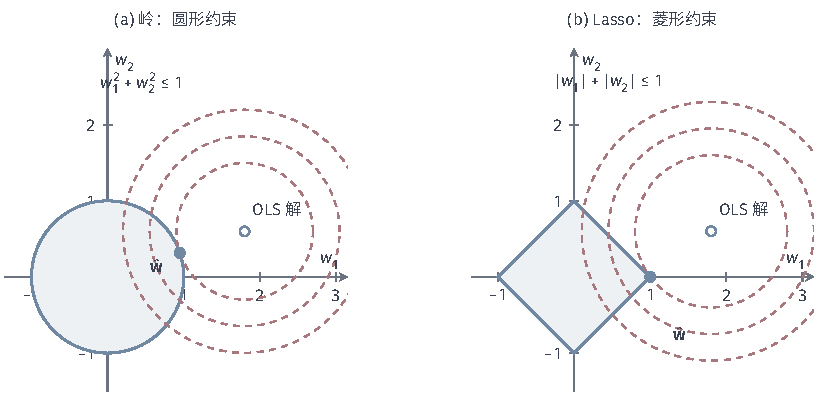
\includegraphics[width=138.649mm]{figures/04-classic-models/00-shared/tikz/regression-regularization-geometry/figure.pdf}
  \caption{岭与Lasso的约束几何。构造损失为$J(\bm{w})=\lVert\bm{w}-(1.8,0.6)^{\top}\rVert_2^2/2$，虚线为等损失线，浅色区域为可行域，空心点为OLS解，实心点为约束最优解。左图解为$(1.8,0.6)^{\top}/\sqrt{3.6}$，右图解为$(1,0)^{\top}$。两图都取单位约束半径以比较形状，不表示相同的惩罚强度；Lasso也并非总在尖点取到最优解。}
  \label{fig:regression-regularization-geometry}
\end{figure*}

\subsubsection{参数学习}
\label{sec:regression-regularization-learning}

\paragraph{岭回归的线性求解}

把平方损失与二次惩罚相加，对参数求梯度并令其为零，得到在OLS正规方程上增加$n\lambda\bm{I}$的移位线性系统，其解为
\begin{equation}
  \widehat{\bm{w}}_{\lambda}
  =(\bm{X}^{\top}\bm{X}+n\lambda\bm{I})^{-1}\bm{X}^{\top}\bm{y},
  \qquad\lambda>0.
  \label{eq:regression-ridge-solution}
\end{equation}
它仍是线性方程，可用直接分解求解；大规模时也可沿梯度迭代更新。恢复截距时使用训练均值$\widehat b=\bar y-\bar{\bm{x}}^{\top}\widehat{\bm{w}}_{\lambda}$。

\paragraph{Lasso的坐标下降}

Lasso目标记为$F(\bm{w})$。固定其余坐标，令$\bm{r}_{-j}=\bm{y}-\sum_{k\ne j}\bm{X}_{:,k}w_k$，$a_j=\lVert\bm{X}_{:,j}\rVert_2^2/n$、$c_j=\bm{X}_{:,j}^{\top}\bm{r}_{-j}/n$，略去常数后的单坐标目标为
\[
  q_j(w_j)=\frac{a_j}{2}w_j^2-c_jw_j+\lambda|w_j|.
\]
正半轴$w_j>0$上导数为$a_jw_j-c_j+\lambda$，驻点$w_j=(c_j-\lambda)/a_j$；负半轴$w_j<0$上导数为$a_jw_j-c_j-\lambda$，驻点$w_j=(c_j+\lambda)/a_j$；零点左侧斜率为$-c_j-\lambda$、右侧为$-c_j+\lambda$，零点最优要求$|c_j|\leq\lambda$。三段合并得到坐标更新
\begin{equation}
  w_j\leftarrow\frac{\mathcal{S}_{\lambda}(c_j)}{a_j},
  \qquad
  \mathcal{S}_{\lambda}(c)=\operatorname{sign}(c)(|c|-\lambda)_+.
  \label{eq:regression-soft-threshold}
\end{equation}
\term{软阈值}（soft thresholding）把阈值内的量置零，将其余量向零移动$\lambda$。循环坐标下降逐个坐标更新，每次更改一个坐标后其余坐标的部分残差必须跟着更新；以次梯度最优性条件的违反程度作为停止依据。

\paragraph{同一设计下的比较与配置}

在正交标准化设计（中心化后$\bm{X}^{\top}\bm{X}/n=\bm{I}_d$）下，各坐标互不交叉：中心化即各列减去自己的样本均值，标准化再除以样本标准差，使各特征量纲一致。$c_j$就是该坐标的OLS参数。此时岭分别除以$1+\lambda$，Lasso分别应用式\eqref{eq:regression-soft-threshold}。例如OLS参数为$(0.12,1.40)$、$\lambda=0.20$，Lasso得到$(0,1.20)$，岭得到$(0.10,1.40/1.20)$，两个坐标都保留。这里比较的是两种惩罚的作用方式，不代表相同数值的$\lambda$给出相同强度的约束。一般相关设计没有消去交叉项的条件，必须反复更新部分残差，不能直接对OLS参数阈值化。超参数选择、特征缩放与变量筛选均在训练折内完成，再由验证折评价。

\subsubsection{理论分析}
\label{sec:regression-regularization-theory}

\paragraph{岭的唯一性与谱收缩}

任意非零$\bm{v}$满足$\bm{v}^{\top}(\bm{X}^{\top}\bm{X}+n\lambda\bm{I})\bm{v}=\lVert\bm{X}\bm{v}\rVert_2^2+n\lambda\lVert\bm{v}\rVert_2^2>0$，所以即使设计秩亏，$\lambda>0$时斜率解也唯一。取SVD$\bm{X}=\bm{U}_r\bm{D}_r\bm{V}_r^{\top}$，正奇异值为$s_j$，则训练预测为
\begin{equation}
  \bm{X}\widehat{\bm{w}}_{\lambda}
  =\sum_{j=1}^{r}\frac{s_j^2}{s_j^2+n\lambda}
       \bm{u}_j\bm{u}_j^{\top}\bm{y}.
  \label{eq:regression-ridge-spectral}
\end{equation}
OLS保留列空间中的全部投影，岭按$s_j^2/(s_j^2+n\lambda)$收缩各谱方向：SVD把设计矩阵拆成互相正交的方向，奇异值$s_j$衡量数据沿该方向铺开的"长度"，$s_j$小意味着数据在该方向几乎没有投影；岭对小奇异值方向的收缩更强，这是稳定性改善的来源，也说明惩罚会同时压低这些方向上的真实信号。比较条件数的对象是正规方程矩阵$\bm{X}^{\top}\bm{X}+n\lambda\bm{I}$，而非$\bm{X}$本身：其极端特征值之比为$(\gamma_{\max}+n\lambda)/(\gamma_{\min}+n\lambda)$，比$\bm{X}^{\top}\bm{X}$的比值更温和。

\paragraph{Lasso的零系数与唯一性}

损失项处处可微，一范数在零点没有普通导数，OLS的“总梯度等于零”不能直接检验。\term{次梯度}（subgradient）用位于凸函数下方的支持直线描述可用斜率：凸函数最优性可统一表为$0\in\partial F(\bm{w})$。对Lasso得到充要条件
\begin{equation}
  \frac{\bm{X}^{\top}(\bm{y}-\bm{X}\widehat{\bm{w}})}{n}
  =\lambda\bm{z},\qquad
  z_j\in
  \begin{cases}
    \{\operatorname{sign}(\widehat w_j)\},&\widehat w_j\ne0,\\
    [-1,1],&\widehat w_j=0.
  \end{cases}
  \label{eq:regression-lasso-kkt}
\end{equation}
非零坐标对应绝对值导数为符号函数，零坐标则允许整个区间抵消损失梯度。需要区分三件事：拟合值唯一、参数唯一、被选变量唯一不是同一命题。两列完全相同且最优参数和为正时，$(a,0)$、$(0,a)$与$(a/2,a/2)$有同样的数据拟合和一范数惩罚，相关变量可以互相替代，轻微扰动就可能改变选择。

\paragraph{预测偏差与估计方差}

在明确的重复抽样条件下，固定未来输入$\bm{x}$，设响应均值为$m(\bm{x})$，未来噪声独立于训练记录且方差有限。把由不同训练集得到的预测再取平均，平方误差分解为
\[
  \begin{aligned}
  \mathbb E[(Y_\star-\widehat f(\bm{x}))^2\mid\bm{x}]
  &=\operatorname{Var}(Y_\star\mid\bm{x})\\
  &\quad+[\mathbb E\widehat f(\bm{x})-m(\bm{x})]^2
   +\operatorname{Var}(\widehat f(\bm{x})).
  \end{aligned}
\]
展开平方后交叉项期望为零，三项分别是未来噪声、平均预测偏离真实均值的偏差平方、以及预测围绕其平均的估计方差。惩罚可能降低最后一项，同时增大中间一项；是否有益要比较两者之和，不能给出无条件的性能排序。图\ref{fig:regression-bias-variance-noise}是这种取舍的教学示意，不是对任意数据的性能排序。

\begin{figure}[htbp]
  \centering
  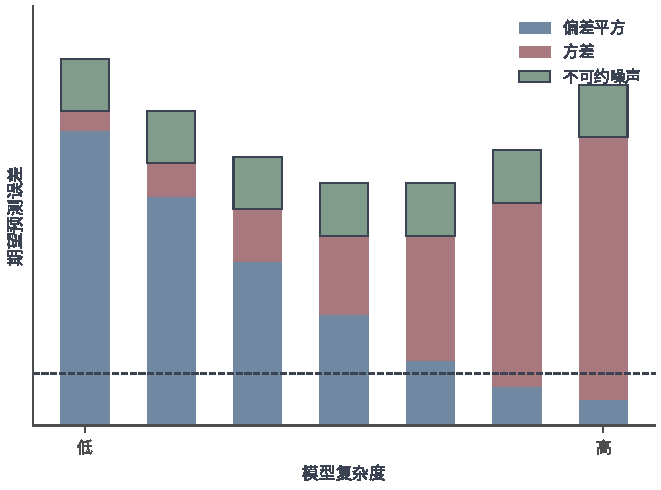
\includegraphics[width=105.412mm]{figures/04-classic-models/00-shared/matplotlib/regression-bias-variance-noise/figure.pdf}
  \caption{模型复杂度变化时的偏差—方差—噪声分解示意。柱高是教学构造的相对量，不来自实验：复杂度增加时偏差平方下降、估计方差上升，不可约噪声保持不变。总误差由三部分共同决定，因此“模型更复杂”与“误差更小”都不是无条件结论。}
  \label{fig:regression-bias-variance-noise}
\end{figure}

\subsubsection{稳定相关变量：弹性网}
\label{sec:regression-elastic-net}

Lasso在特征高度相关时会在完全相同的两列之间任意择一，数据难以决定保留哪个变量。\term{弹性网}（elastic net）在一范数之外加入二次惩罚，目标为
\[
  \frac{1}{2n}\lVert\bm{y}-\bm{X}\bm{w}\rVert_2^2
  +\lambda_1\lVert\bm{w}\rVert_1
  +\frac{\lambda_2}{2}\lVert\bm{w}\rVert_2^2,
\]
两个强度参数$\lambda_1,\lambda_2\geq0$分别控制坐标稀疏与稳定分摊，常取$\lambda_1=\lambda\alpha$、$\lambda_2=\lambda(1-\alpha)$，$0\leq\alpha\leq1$。Zou与Hastie在2005年研究了这一结合；原始文献还讨论了对参数重标定以修正过度收缩的版本\scite{zou2005elastic}。

在Lasso的坐标子问题上增加二次项后，$a_j$变为$a_j+\lambda_2$，更新改为$\mathcal{S}_{\lambda_1}(c_j)/(a_j+\lambda_2)$。截距仍按训练均值恢复，两个强度由训练内验证共同选择。两列完全相同时，二次项使平均分摊的平方范数最小，解在$\lambda_2>0$下唯一；但不同软件中$\lambda$的系数约定不同，同数值不等于同强度，跨软件比较前应把平方损失与惩罚换算到相同约定。

\subsubsection{支持成组选择：组Lasso与稀疏组Lasso}
\label{sec:regression-group-lasso}

\paragraph{组Lasso}

另一些变量由多个参数共同表示：一个分类字段展开成多个指示变量，或一组传感器读数合起来才是一个测量通道；选择问题是“是否保留整组”，而不是“是否保留某次展开”。\term{组Lasso}（group Lasso）把预先指定的一组坐标作为选择单位，惩罚为
\[
  \lambda\sum_{g=1}^{G}\omega_g\lVert\bm{w}_{A_g}\rVert_2,
\]
其中$A_1,\ldots,A_G$是不重叠且覆盖全部斜率坐标的组，$\omega_g>0$为组权重，常取$\sqrt{|A_g|}$。组向量为零意味着整组作用被删除；保留一组则允许各参数共同拟合其形状，组内某些坐标仍可为零。Yuan与Lin在2006年研究了这种成组变量选择\scite{yuan2006group}。

记光滑数据项$g(\bm{w})=\lVert\bm{y}-\bm{X}\bm{w}\rVert_2^2/(2n)$。近端梯度把不可导的组范数留在显式步骤里：先沿光滑项$g$的梯度走一步，再对惩罚做阈值化。先用二次函数在当前点附近从上方近似$g$，得到近端子问题$\min_{\bm{u}}\lVert\bm{u}-\bm{v}_{A_g}\rVert_2^2/2+t\lambda\omega_g\lVert\bm{u}\rVert_2$，其中$\bm{v}=\bm{w}-t\nabla g(\bm{w})$。把同向候选写成$\bm{u}=r\bm{v}_{A_g}/\lVert\bm{v}_{A_g}\rVert_2$，$r\geq0$，标量目标为
\[
  \tfrac12(r-\lVert\bm{v}_{A_g}\rVert_2)^2+t\lambda\omega_g r.
\]
内部驻点$r=\lVert\bm{v}_{A_g}\rVert_2-t\lambda\omega_g$为负时约束最小点在$r=0$，合并得径向阈值
\begin{equation}
  \bm{w}_{A_g}^{+}
  =
  \begin{cases}
    \bm{0},&\lVert\bm{v}_{A_g}\rVert_2\leq t\lambda\omega_g,\\
    \left(1-\dfrac{t\lambda\omega_g}{\lVert\bm{v}_{A_g}\rVert_2}\right)
      \bm{v}_{A_g},&\text{其他情形}.
  \end{cases}
  \label{eq:regression-group-prox}
\end{equation}
该闭式解针对欧氏距离构成的近端子问题；一般设计的块坐标子问题还包含组内设计的曲率，需要据此求解。对非零设计取$0<t\leq1/\lVert\bm{X}^{\top}\bm{X}/n\rVert_2$可保证凸近端梯度法的目标收敛。

\paragraph{稀疏组Lasso}

整组筛选之后仍可能需要删除组内部分坐标，\term{稀疏组Lasso}（sparse group Lasso）在组范数之外再加一范数$\lambda_1\lVert\bm{w}\rVert_1$。固定一次梯度步后，先对每个坐标作阈值$t\lambda_1$的软阈值，再按组作阈值$t\lambda\omega_g$的径向阈值；两步分别对应坐标近端子问题与组近端子问题。面对同一批候选组，Lasso逐坐标选择、组Lasso整组取舍、稀疏组Lasso先选组再在组内选择，三者保留的对象不同。组内选择、相关变量替代与配置验证的条件仍需在训练折内检查，正则强度由训练内验证选择。
